\documentclass{standalone}

\usepackage[utf8]{inputenc}
\usepackage{tikz}

\begin{document}
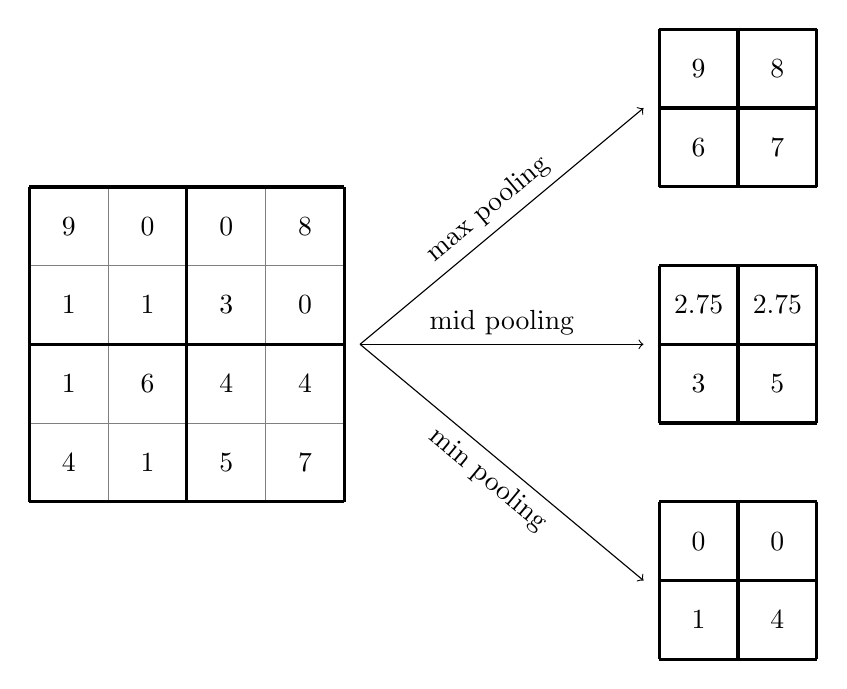
\begin{tikzpicture}
  \def\margin{2cm}
  \tikzset{block grid/.style={very thick}}
  \begin{scope}[xshift=-4cm-\margin,yshift=-2cm]
    \draw[help lines] (0, 0) grid (4, 4);
    \draw[block grid] (0, 0) grid [step=2cm] (4, 4);
    \foreach \row [count=\j] in {%
      {9,0,0,8},%
      {1,1,3,0},%
      {1,6,4,4},%
      {4,1,5,7}%
    } {
      \foreach \cell [count=\i] in \row {
        \node at (\i - 0.5, 4 - \j + 0.5) {\cell};
      }
    }
  \end{scope}
  \draw [->] (-1.8, 0) to node[above, sloped] {max pooling} (1.8, 3);
  \begin{scope}[xshift=\margin,yshift=2cm]
    \draw[block grid] (0, 0) grid (2, 2);
    \foreach \row [count=\j] in {{9,8},{6,7}} {
      \foreach \cell [count=\i] in \row {
        \node at (\i - 0.5, 2 - \j + 0.5) {\cell};
      }
    }
  \end{scope}
  \draw [->] (-1.8, 0) to node[above] {mid pooling} (1.8, 0);
  \begin{scope}[xshift=\margin,yshift=-1cm]
    \draw[block grid] (0, 0) grid (2, 2);
    \foreach \row [count=\j] in {{2.75,2.75},{3,5}} {
      \foreach \cell [count=\i] in \row {
        \node at (\i - 0.5, 2 - \j + 0.5) {\cell};
      }
    }
  \end{scope}
  \draw [->] (-1.8, 0) to node[below, sloped] {min pooling} (1.8, -3);
  \begin{scope}[xshift=\margin,yshift=-4cm]
    \draw[block grid] (0, 0) grid (2, 2);
    \foreach \row [count=\j] in {{0,0},{1,4}} {
      \foreach \cell [count=\i] in \row {
        \node at (\i - 0.5, 2 - \j + 0.5) {\cell};
      }
    }
  \end{scope}
\end{tikzpicture}
\end{document}
